\chapter{Конструкторская часть}
В данной части будут реализованы блок-схемы алгоритмов поиска максимального числа в последовательности, произведена оценка их трудоёмкости и затрачиваемая памяти.

\section{Описание алгоритмов}
На основе аналитической части были спроектированы алгоритмы умножения матриц. Блок-схемы этих алгоритмов приведены на рисунке 2.1 (стандартный), рисунке 2.2 (Винограда) и рисунке 2.3 (Оптимизированного Винограда).


\begin{figure}[H]
	\centering
	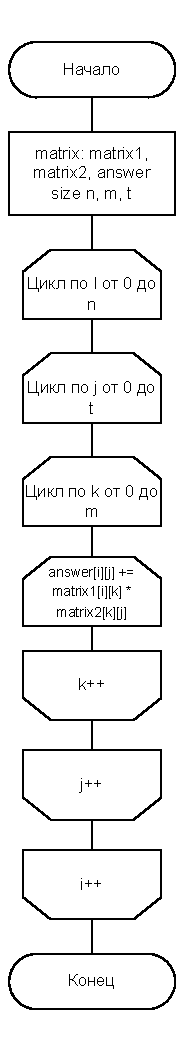
\includegraphics[width=0.18\textwidth]{images/AA1_1.pdf}
	\caption{Схема стандартного алгоритма умножения матриц}
	\label{fig:example_1}
\end{figure}

\begin{figure}[H]
	\centering
	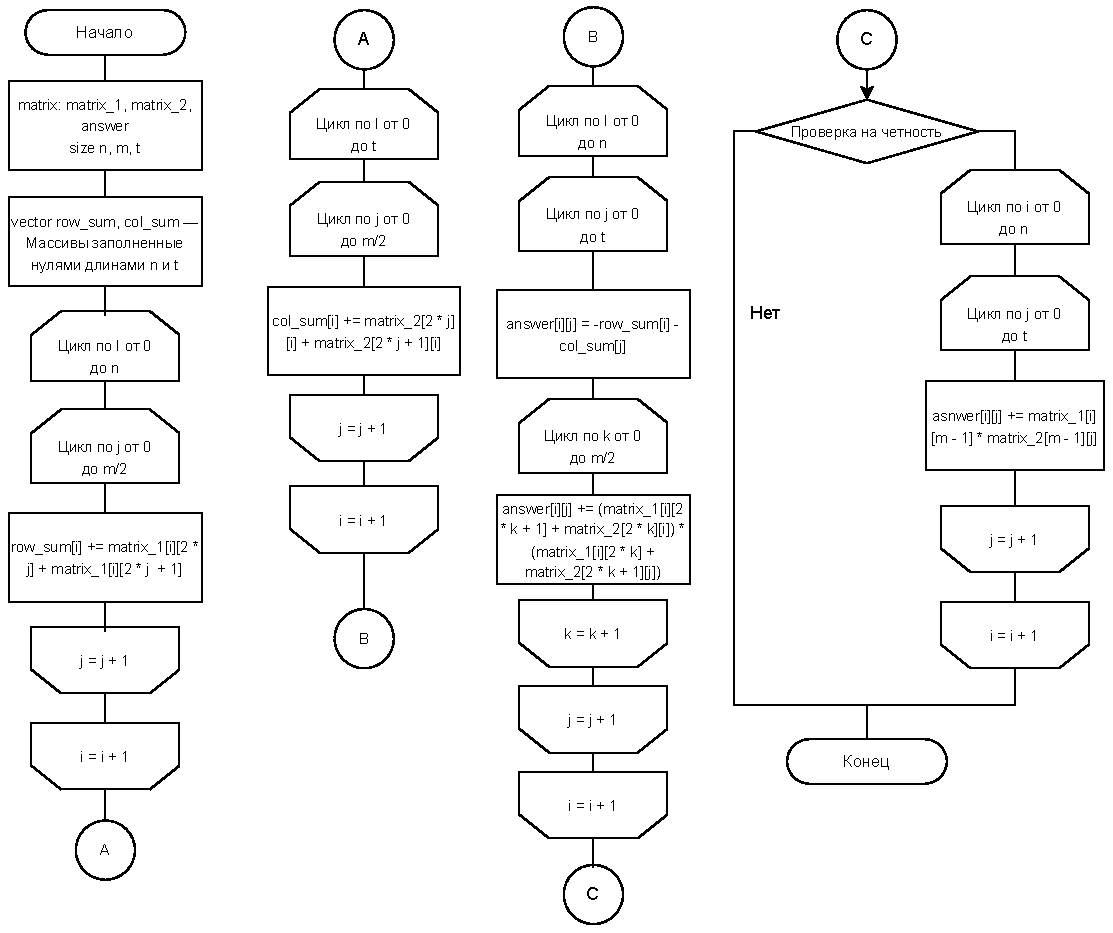
\includegraphics[width=0.8\textwidth]{images/AA1_2.pdf}
	\caption{Схема алгоритма Винограда}
	\label{fig:example_2}
\end{figure}

\begin{figure}[H]
	\centering
	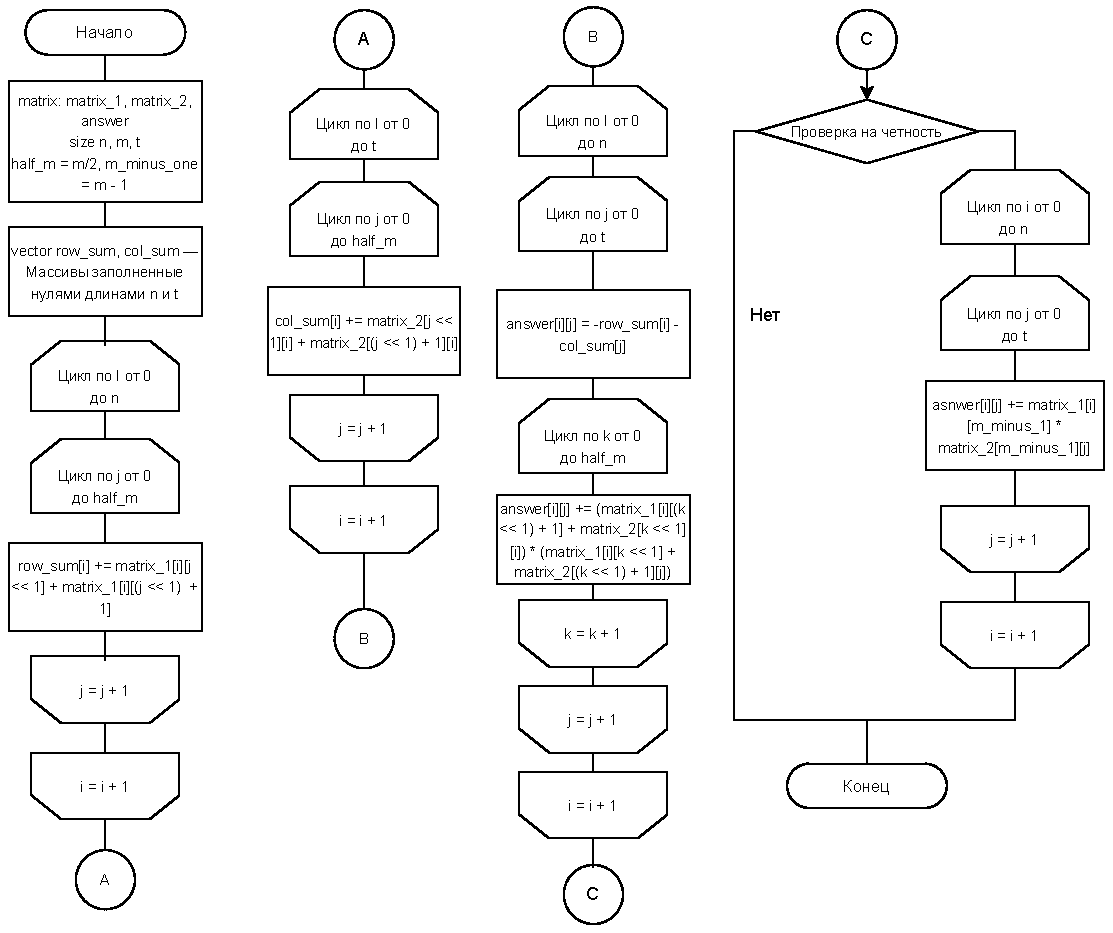
\includegraphics[width=0.8\textwidth]{images/AA1_3.pdf}
	\caption{Схема алгоритма Винограда}
	\label{fig:example_3}
\end{figure}
\section{Оценка трудоёмкости алгоритмов}
Введена модель для оценки трудоёмкости

\begin{enumerate}
	\item Трудоёмкость базовых операций
    \begin{itemize}
	\item Определим трудоёмкость следующих операций равной 1:\\
	\( + \), \( - \), \( ! \), \( != \), \( == \), \( \neq \), \( \leq \), \( \geq \), \( > \), \( < \), \( += \), \( -= \), \( []\), \( || \), \( \&\& \), \( << \)
	\item Определим трудоёмкость следующих операция равной 2:\\
	\( * \), \( / \), \( *= \), \( /= \), \( \% \)
\end{itemize}
	\item Трудоёмкость циклов
	\begin{equation}\label{eq:cycle_complexity}
		f = f_{\text{иниц.}} + f_{\text{сравн.}} + N_{\text{итер}} \cdot (f_{\text{тела}} + f_{\text{инкремента}} + f_{\text{сравн.}})
	\end{equation}
	\item Трудоёмкость условного оператора, приняв трудоёмкость условного перехода за ноль
	\begin{equation}\label{eq:if_complexity}
		f_{\text{if}} = f_{\text{условия}} + \begin{cases}
			\min(f_{\text{true}}, f_{\text{false}}), & \text{в лучшем случае} \\
			\max(f_{\text{true}}, f_{\text{false}}), & \text{в худшем случае}
		\end{cases}
	\end{equation}
\end{enumerate}

\section{Трудоёмкость стандартного алгоритма}
Трудоёмкость стандартного алгоритма состоит из :
\begin{itemize}
\itemтрудоёмкость цикла по \(i \) от \( 1 \) до \(n \): \begin{equation}f = 2 + n * (2 + f_{body})  \end{equation}
\itemтрудоёмкость цикла по \(j\) от \( 1 \) до \(t \): \begin{equation}f = 2 + t * (2 + f_{body})  \end{equation}
\item трудоёмкость цикла по \(k\) от \( 1 \) до \(m \): \begin{equation}f = 2 + k * (2 + f_{body})  \end{equation}
\itemтрудоёмкость тела цикла по \(k\): \begin{equation}f = 2 + 1 + 2 + 2 + 2 = 11
   \end{equation}
\end{itemize}

Таким образом, общая трудоёмкость равна
 \begin{equation}f = 2 + n * (2 + 2 + t * (2 + 2 + 11k) \end{equation}
  \begin{equation}f = 2 + n * (4 + t * (4 + 11k) =  2  + n * (4 + 4t +11tk) \end{equation}
   \begin{equation}f = 11ntk + 4nt + 4n + 2 \approx ntk \approx O(N^3) \end{equation}

\section{Трудоёмкость алгоритма Винограда}
Трудоёмкость стандартного алгоритма состоит из :
\begin{itemize}
	\itemвыделение памяти и инициализация векторов:  \begin{equation}f =  17nm/2 + 17tm/2 + 6t + 6n + 4  \end{equation}
	\itemтрудоёмкость цикла по \(i\) от \( 1 \) до \(n \): \begin{equation}f = 2 + n * (2 + f_{body})  \end{equation}
	\itemтрудоёмкость цикла по \(j\) от \( 1 \) до \(t \): \begin{equation}f = 2 + t * (9 + f_{body})  \end{equation}
	\item трудоёмкость цикла по \(k\) от \( 1 \) до \(m / 2 \): \begin{equation}f = 2 + 27 * m/2  \end{equation}
	\item трудоёмкость проверки на нечетность
	\begin{equation}\label{eq:if_complexity}
		f_{\text{if}} = 3 + \begin{cases}
			0, & \text{в лучшем случае} \\
			13nt + 4n + 2, & \text{в худшем случае}
		\end{cases}
	\end{equation}
\end{itemize}
Таким образом, общая трудоёмкость равна:
\begin{equation}\label{eq:if_complexity}
	f = \begin{cases}
		27nmt/2 + 17nm/2 + 17tm/2 + 11nt + 6t + 10n + 6, & \text{в лучшем случае} \\
		27nmt/2 + 17nm/2 + 17tm/2 + 24nt + 6t + 14n + 8 & \text{в худшем случае}
	\end{cases}
\end{equation}
\begin{equation}f = 13.5nmt + 8.5nm + 8.5mt + 24nt \approx O(N^3) \end{equation}

\section{Трудоёмкость оптимизированного алгоритма Винограда}
Трудоёмкость стандартного алгоритма состоит из :
\begin{itemize}
	\itemинициализация переменных: \begin{equation*}f = 3\end{equation*}
	\itemвыделение памяти и инициализация векторов:  \begin{equation}f = 13nm/2 + 13tm/2 + 4n + 4t + 4 \end{equation}
	\item трудоёмкость цикла по \(i\) от \( 1 \) до \(n \): \begin{equation}f = 2 + n * (2 + f_{body})  \end{equation}
	\itemтрудоёмкость цикла по \(j\) от \( 1 \) до \(t \): \begin{equation}f = 2 + t * (9 + f_{body})  \end{equation}
	\item трудоёмкость цикла по \(k\) от \( 1 \) до \(m / 2 \): \begin{equation}f = 2 + m/2 * (2 + f_{body})  \end{equation}
	\itemтрудоёмкость тела цикла  \begin{equation}f = 2 + 1 + 2 + 1 + 1 + 1 + 2 + 1 + 2 + 2 + 1 + 1 + 2 + 1 + 1 = 21 \end{equation}
	\item трудоёмкость проверки на нечетность
		\begin{equation}\label{eq:if_complexity}
		f_{\text{if}} = 3 + \begin{cases}
			0, & \text{в лучшем случае} \\
			11nt + 4n + 5, & \text{в худшем случае}
		\end{cases}
	\end{equation}
\end{itemize}

Таким образом, общая трудоёмкость равна
\begin{equation}f = 13nm/2 + 13tm/2 + 4n + 4t + 6 + n * (4 + t * (11 + m/2 * 23)) \end{equation}
\begin{equation}f = 13nm/2 + 13tm/2 + 4n + 4t + 6 + n * (4 + 11t + 23tm/2) \end{equation}
\begin{equation}f = 13nm/2 + 13tm/2 + 4n + 4t + 6 + 4n + 11tn + 23tmn/2 \end{equation}
\begin{equation}f = 23tmn/2 + 13nm/2 + 13tm/2 + 11tn + 4t + 8n + 6 \end{equation}

\begin{equation}\label{eq:if_complexity}
	f = \begin{cases}
		23tmn/2 + 13nm/2 + 13tm/2 + 11tn + 4t + 8n + 9, & \text{в лучшем случае} \\
		23tmn/2 + 13nm/2 + 13tm/2 + 22nt + 4t + 12n + 11 & \text{в худшем случае}
	\end{cases}
\end{equation}
\begin{equation}f = 11.5nmt + 6.5nm + 6.5mt + 11 nt \approx O(N^3) \end{equation}

\section{Используемые типы данных}
При реализации алгоритмов использовались следующие типы данных:
\begin{itemize}
	\itemразмеры матрицы: \text{size\_t};
	\itemтип данных матрицы: int;
	\itemтип данных вспомогательных векторов: int;
\end{itemize}

\section{Оценка памяти}
Пусть matrix — матрица целых чисел
\begin{itemize}
\item размерность входных матриц \( n * m\) и \(m * t\);
\item размерность результирующей матрицы \(n * t\);
\end{itemize}
Для стандартного алгоритма умножения будет затрачена память на:
\begin{itemize}
\item размеры матрицы — \(3 * sizeof\text(size\_t)\);
\item матрицы —  \((n* m + m * t + n * t) * sizeof(int)\);
\end{itemize}
Для алгоритма Винограда создаются два дополнительных массива, для
которых используется \((n + t) * sizeof(int)\) памяти. Для оптимизации алгоритма используется две вспомогательные переменные размером \(sizeof\text(size\_t)\).

В стандартном алгоритме не используется дополнительная памяти на массивы, что даёт ему выигрыш по сравнению с алгоритмом Виноградова, хоть и незначительный.

\section{Структура программы}
Программное обеспечение будет состоять из нескольких частей:
\begin{itemize}
	\itemглавный модуль — предоставляет возможность выбора режима работы программы, а также обеспечивает запуск программы;
	\itemинтерфейс — модуль для взаимодействия пользователя с программой. Пользователь может выбрать режим работы, а также ввести входные данные для умножения матриц или тестовых замеров;
	\itemмодуль, содержащий функции для работы с матрицами — предоставляет возможность объявить, проинициализировать, прочитать, заполнить случайными числами и совершить арифметические операции над типом данных;
	\itemмодуль для совершения замеров процессорного времени выполнения умножения матриц;
\end{itemize}

\section*{Вывод}
На основе аналитической части были реализованы блок-схемы алгоритмов умножения матриц, произведена оценка их трудоёмкости, вычислена затрачиваемая памяти, под каждый анализ, а также продуманы модули программ.

\clearpage
